\documentclass[a4paper]{article}
 
% - taille de la fonte    : 10pt, 11pt, 12pt
% - recto ou recto-verso    : oneside, twoside
 
% Chargement d'extensions
%\usepackage[latin1]{inputenc}    
\usepackage[francais]{babel}    
\AtBeginDocument{\def\labelitemi{$\bullet$}}

\usepackage{amsmath}
\makeatletter
%%%%%%%%%%%%%%%%%%% debut fichier boiboites.sty %%%%%%%%%%%%%%%%%%%%%%
\RequirePackage{xkeyval}
\RequirePackage{tikz}
\RequirePackage{amssymb}

\define@key{boxedtheorem}{titlecolor}{\def\titlecolor{#1}}
\define@key{boxedtheorem}{titlebackground}{\def\titlebackground{#1}}
\define@key{boxedtheorem}{background}{\def\background{#1}}
\define@key{boxedtheorem}{titleboxcolor}{\def\titleboxcolor{#1}}
\define@key{boxedtheorem}{boxcolor}{\def\boxcolor{#1}}
\define@key{boxedtheorem}{thcounter}{\def\thcounter{#1}}
\define@key{boxedtheorem}{size}{\def\size{#1}}
\presetkeys{boxedtheorem}{titlecolor = black, titlebackground = white, background = white,%
                         titleboxcolor = black, boxcolor = black, thcounter=, size = .9\textwidth}{}

\newcommand{\couleurs}[1][]{%
    \setkeys{boxedtheorem}{#1}
    \tikzstyle{fancytitle} =[draw=\titleboxcolor, rounded corners, fill=\titlebackground,
                            text= \titlecolor]
    \tikzstyle{mybox} = [draw=\boxcolor, fill=\background, very thick,
                        rectangle, rounded corners, inner sep=10pt, inner ysep=20pt]
}


%Commande generique pour faire un joli encadre
\newsavebox{\boiboite}
\newcommand{\titre}{Titre}
\newenvironment{boite}[2][]%
    {%
    \renewcommand{\titre}{#2}
    \couleurs[#1]
    \begin{lrbox}{\boiboite}%
     \begin{minipage}[!h]{\size}
    }%
    {%
     \end{minipage}
    \end{lrbox}
    \begin{center}
    \begin{tikzpicture}
    \node [mybox] (box){\usebox{\boiboite}};
    \node[fancytitle, right=10pt] at (box.north west) {\titre};
    \end{tikzpicture}
    \end{center}
    }

\newcommand{\newboxedtheorem}[4][]{%
    \couleurs[#1]
    \@ifnotempty{#4}{%
      \@ifundefined{the#4}{\@ifundefined{\thcounter}{\newcounter{#4}}{%
      \newcounter{#4}[\thcounter ] } } { }%
    }
    \newenvironment{#2}[1][]{%
    \@ifnotempty{#4}{\refstepcounter{#4}}
    \begin{boite}[#1]{\textbf{#3\@ifnotempty{#4}{ \csname the#4\endcsname}}\@ifnotempty{##1}{
    (##1)}}
    }%
    {%
    \end{boite}
    }
}
%%%%%%%%%%%%%%%%%%%% end fichier boiboites.sty %%%%%%%%%%%%%%%%%%%%%%
\makeatother
\newboxedtheorem{theorem}{}{theorem}
%%%%%%%%%% hypertext

\usepackage{hyperref}
\hypersetup{
    colorlinks=true,
    linkcolor=blue,
    filecolor=magenta,      
    urlcolor=cyan,
    pdftitle={Overleaf Example},
    pdfpagemode=FullScreen,
    }

\urlstyle{same}

%%%%%%%%%%%%%%%%%%%%%%%%%%%
\usepackage{amsthm}
%\usepackage{amsmath}
\usepackage{amssymb}
\usepackage{mathrsfs}
\usepackage{graphicx}
\usepackage{geometry}
\usepackage{stmaryrd}
\usepackage{tikz}
\usetikzlibrary{patterns}

\usepackage[cache=false]{minted}
\usepackage{xcolor}
%\setbeamercolor{background canvas}{bg=lightgray}
\definecolor{LightGray}{gray}{0.9}
\definecolor{monOrange}{rgb}{0.97,0.35,0.04}

% Informations le titre, le(s) auteur(s), la date
\title{Vue3}
\author{Ibrahim ALAME}
\date{\today}
\includeonly{ introduction.tex} 
\begin{document}
 
\maketitle
 %Mettez en place une API simple avec Django REST Framework
 \section{Découvrez Django REST Framework}
 \subsection{Découvrez pourquoi utiliser une API}
 Grosso modo, c’est quelque chose qui permet de communiquer facilement avec tout un système d’information. On actionne un levier et bim ça fait ce qu’on veut derrière (il s’annonce bien ce cours !). Mais on va quand même voir ce qu’est un levier, et surtout comment on l’actionne, rassurez-vous !

{\color{monOrange}API} signifie {\em Application Programming Interface} (ou {\em interface de programmation applicative}). C’est une grosse interface qui permet d'interagir avec un système d’information au travers de ce qu’on appelle des endpoints. Chaque endpoint permet d’exécuter différentes actions dans le système d’information, sans avoir à en comprendre le fonctionnement. Ces actions peuvent être la consultation d’un panier, l’envoi d’un e-mail, l’authentification auprès d’un service… les possibilités sont nombreuses.
\begin{theorem}
En gros, c’est un peu comme utiliser une classe fournie par une librairie tierce. C’est-à-dire qu’on utilise des méthodes d'objets de cette librairie que nous n’avons pas écrites nous-même. Dans notre cas, la classe est le système d’information, et la méthode est l'endpoint.
\end{theorem}
\subsubsection*{Mais concrètement, un endpoint, c’est quoi ?}
Un endpoint est une URL sur laquelle on réalise différents appels. Selon la méthode HTTP utilisée (GET, POST, PATCH, DELETE), une partie de code va être exécutée et retourner un résultat. Ce résultat est constitué :
\begin{itemize}
\item D’un status code (200, 201, 400, etc.) qui indique le succès ou non de l’appel ;
\item D’un contenu qui est en JSON dans la majorité des cas (peut également être du XML dans certains cas), et qui va contenir des informations soit de succès soit d’erreur.
Ces appels peuvent ensuite être paramétrés avec des filtres dans les paramètres d’URL ou dans le corps de la requête.
\end{itemize}

Les API sont aujourd’hui devenues un standard. Elles permettent de centraliser toute l’information en ayant moins de données et de logique métier à gérer dans les terminaux. Une seule application Backend proposant une API peut être mutualisée et être consommée par une application Front, des applications mobiles Android/iOS, mais aussi d’autres systèmes d’information, des partenaires, etc.

\begin{center}
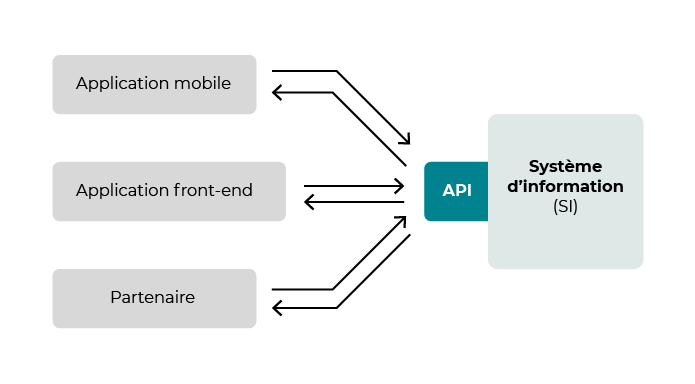
\includegraphics[width=10cm]{images/image01.png}
\end{center}

Une API peut être créée dès le début d’un projet, mais aussi être mise en place sur un projet existant pour le faire évoluer. C’est ce dernier que nous allons ensuite voir ensemble, en {\bf adaptant un projet Django existant pour lui intégrer une API avec {\color{monOrange}Django REST Framework}} (DRF).
\subsection{Découvrez le cas concret du cours}
Tout au long de ce cours, nous allons {\em mettre en place une {\color{monOrange}API}} sur un projet de boutique en ligne qui permet à des utilisateurs de consulter un catalogue de produits rangé par catégories, produits et articles. 

Nous permettrons ensuite aux {\color{monOrange}administrateurs de la plateforme de gérer la boutique} en ligne, en ajoutant de nouveaux produits à mettre en vente, et en masquant certains produits s’ils ne sont plus disponibles. Nous devrons alors sécuriser certains endpoints pour qu’ils ne soient pas accessibles publiquement.

Le code de l’application est disponible sur ce repository. À la fin de certains chapitres, des exercices seront proposés en partant d’une branche {\color{monOrange}Git}, et une solution sera proposée dans une autre branche.
\subsection{Installez et configurez {\color{monOrange}DRF}}
Django REST Framework est une librairie permettant la mise en place d’une API pour Django (vous pouvez regarder sa documentation sur le site officiel, en anglais). Basée sur le framework, elle propose la mise en place des endpoints d’une façon similaire à la mise en place des URL, Views et Forms de Django.
\subsubsection*{Pourquoi utilise-t-on cette librairie ?}
Écrire une API à la main est possible, on pourrait écrire nous-mêmes nos endpoints en nous basant sur les Views de Django, et retourner du JSON.

Mais c’est en réalité une quantité de travail phénoménale, et d’autres développeurs se sont déjà penchés sur le sujet pour simplifier grandement l’écriture d’API.

Dans ce chapitre, nous allons faire simple et :
\begin{itemize}
\item Mettre en place la librairie, en l’ajoutant aux dépendances de notre projet ;
\item Déclarer DRF parmi les applications du projet Django pour permettre son utilisation ;
\item Configurer une première URL fournie par DRF pour s’assurer du bon fonctionnement de la librairie.
\end{itemize}
En partant de la \href{https://github.com/OpenClassrooms-Student-Center/7192416_APIs_DRF}{branche main de notre projet},
\begin{center}
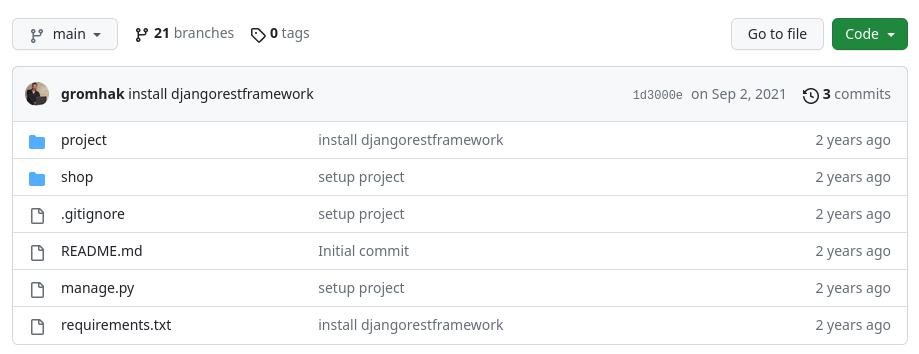
\includegraphics[width=10cm]{images/image02.png}
\end{center}
\begin{center}

\includegraphics[width=10cm]{images/image03.png}
\end{center}
 commençons par {\bf ajouter la dépendance à DRF} dans notre fichier {\color{monOrange}requirements.txt}  :
\begin{minted}[
mathescape,
framesep=2mm,
baselinestretch=1.2,
%fontsize=\footnotesize,
bgcolor=LightGray,
%linenos
]{latex}
djangorestframework==3.12.4
\end{minted}

Un petit coup d’ install  dans notre environnement virtuel :
\begin{minted}[
mathescape,
framesep=2mm,
baselinestretch=1.2,
%fontsize=\footnotesize,
bgcolor=LightGray,
%linenos
]{bash}
pip install -r requirements.txt
\end{minted}

Puis, déclarons DRF dans la liste des applications installées du fichier  settings.py  du projet Django :
\begin{minted}[
mathescape,
framesep=2mm,
baselinestretch=1.2,
%fontsize=\footnotesize,
bgcolor=LightGray,
%linenos
]{python}
INSTALLED_APPS = [
'rest_framework',
]
\end{minted}

Pour nous assurer que notre API est fonctionnelle, nous allons activer l’authentification fournie par DRF pour nous connecter. Éditons notre fichier  urls.py  :
\begin{minted}[
mathescape,
framesep=2mm,
baselinestretch=1.2,
%fontsize=\footnotesize,
bgcolor=LightGray,
%linenos
]{python}
urlpatterns = [
    path('api-auth/', include('rest_framework.urls'))
]
\end{minted}

Démarrons à présent notre serveur de développement et allons nous connecter sur notre API à présent en place :
\begin{minted}[
mathescape,
framesep=2mm,
baselinestretch=1.2,
%fontsize=\footnotesize,
bgcolor=LightGray,
%linenos
]{bash}
python manage.py runserver
\end{minted}

Nous devrions maintenant pouvoir nous rendre sur notre URL et nous connecter. Le projet contient une base de données SQLite qui contient déjà un compte administrateur dont voici les identifiants :
\begin{itemize}
\item Nom d’utilisateur : admin-oc
\item Mot de passe : password-oc
\end{itemize}

Le projet étant en local, nous pouvons nous connecter à l’URL

\url{http://127.0.0.1:8000/admin}.

Nous avons installé et configuré DRF !
\begin{center}
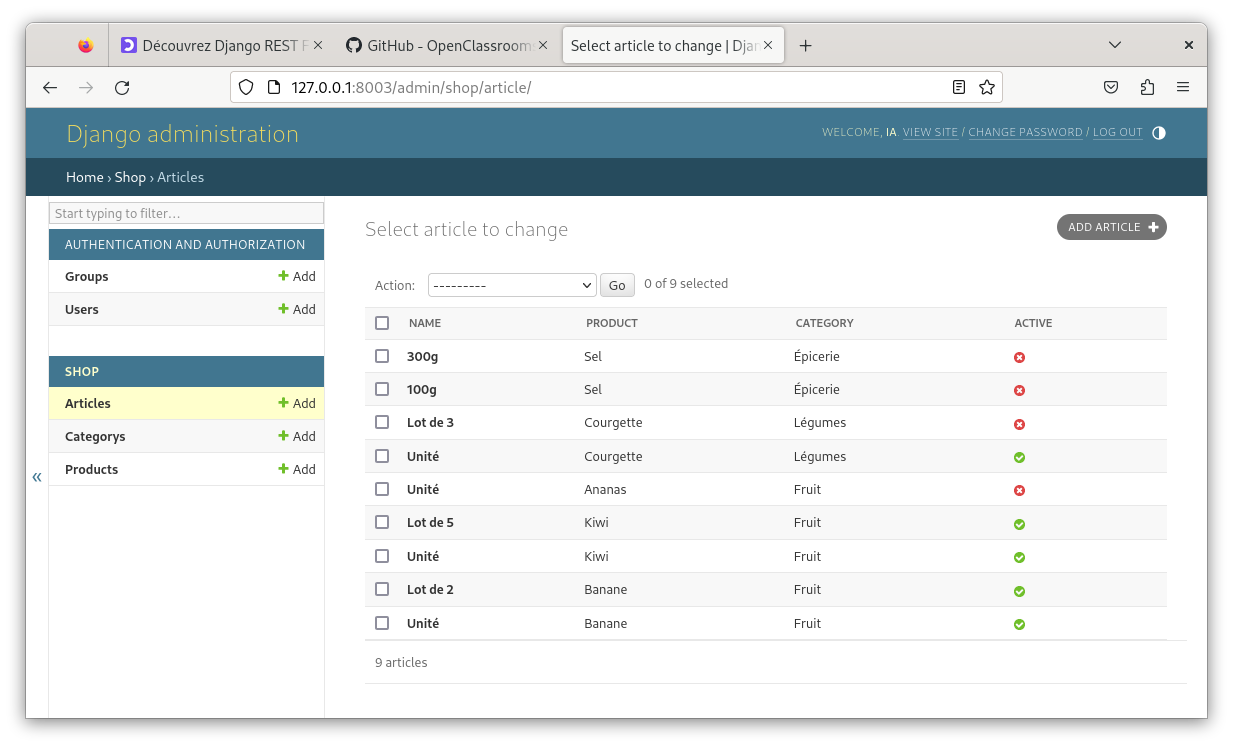
\includegraphics[width=15cm]{images/image04.png}
\end{center}
\subsubsection*{En résumé}
\begin{itemize}
\item Les API sont des interfaces permettant l’échange et le traitement d’informations entre un système d’information et toute autre application.
\item Un endpoint est une URL sur laquelle on peut effectuer des opérations en fonction de la méthode HTTP utilisée.
\item Django Rest Framework est une librairie permettant de mettre en place une API sur un projet Django.
\end{itemize}

{\em Maintenant, on est prêts pour la suite, et sans attendre on va mettre en place notre premier endpoint !}

\section{Gérez des données avec un endpoint}
\subsection{Créez un premier endpoint}
En avant, mettons en place ce premier {\color{monOrange}endpoint} en permettant à nos visiteurs d’accéder à la liste des catégories de nos produits. La toute première chose à faire lors de la réalisation d’un endpoint est de se demander {\bf quelles sont les informations importantes que nous souhaitons en tirer}.

Dans notre cas, pour afficher la liste des catégories, nous allons avoir besoin de leur nom, mais également de leur {\color{monOrange}identifiant}. L’identifiant sera utile aux clients (application front, mobile…) pour identifier de manière claire et unique les catégories s’ils ont des actions à faire dessus, comme afficher les produits qui constituent une catégorie.

DRF met à notre disposition des {\color{monOrange}serializers} qui permettent de transformer nos models Django en un autre format qui, lui, est exploitable par une API. Lorsque notre API sera consultée, le {\em serializer} va nous permettre de transformer notre objet en un JSON et, inversement, lorsque notre API va recevoir du JSON, elle sera capable de le transformer en un objet.

Pour le développeur qui les utilise, ils fonctionnent à la manière des formulaires proposés par Django. C'est-à-dire qu’ils sont paramétrés en précisant le model à utiliser et les champs de ce model à sérialiser.

\begin{theorem}
Pour rappel, un {\tt modelDjango} est une classe matérialisée dans la base de données, et qui permet donc l’utilisation de l’Object-Relational Mapping ({\color{monOrange}ORM}) de Django. Il sert à représenter et faire persister les données métier de notre système d’information. Dans notre cas, il s’agit des catégories, produits et articles mis en vente sur notre boutique.
\end{theorem}
Créons un fichier  {\tt serializers.py}  et {\em écrivons notre premier {\color{monOrange}serializer}}, que nous nommerons  {\tt CategorySerializer}  pour rester clair et précis. ;)

Il est nécessaire de définir sa classe  {\tt Meta}  et la liste des champs, exactement comme pour un formulaire. De plus, les noms des attributs sont identiques.
\begin{minted}[
mathescape,
framesep=2mm,
baselinestretch=1.2,
%fontsize=\footnotesize,
bgcolor=LightGray,
%linenos
]{python}
from rest_framework.serializers import ModelSerializer
from shop.models import Category
 
class CategorySerializer(ModelSerializer):
    class Meta:
        model = Category
        fields = ['id', 'name']

\end{minted}
Occupons-nous à présent de la {\color{monOrange}View}. {\bf DRF} nous propose une  {\color{monOrange}APIView}  qui a également un fonctionnement similaire aux  {\tt Views}  de Django.

Nous devons réécrire la méthode  {\color{monOrange}get}  qui réalisera les actions suivantes :
\begin{itemize}
\item Récupérer toutes les catégories en utilisant l’ORM de Django ;
\item Sérialiser les données à l’aide de notre serializer ;
\item Renvoyer une réponse qui contient les données sérialisées.
\end{itemize}
\begin{minted}[
mathescape,
framesep=2mm,
baselinestretch=1.2,
%fontsize=\footnotesize,
bgcolor=LightGray,
%linenos
]{python}
from rest_framework.views import APIView
from rest_framework.response import Response
from shop.models import Category
from shop.serializers import CategorySerializer
 
class CategoryAPIView(APIView):
    def get(self, *args, **kwargs):
        categories = Category.objects.all()
        serializer = CategorySerializer(categories, many=True)
        return Response(serializer.data)
\end{minted}
Le paramètre  {\color{monOrange}many}  permet de préciser au {\color{monOrange}Serializer} qu’il va devoir générer une liste d’éléments à partir de l’itérable (notre {\color{monOrange}queryset}) qui lui est transmis.

\subsubsection*{Et si je n’ai qu’un seul élément à sérialiser ?}
Dans ce cas, il n’est pas nécessaire de préciser le paramètre  {\color{monOrange}many}, et l’objet peut directement être donné au {\color{monOrange}Serializer} sans le mettre dans un {\em itérable}. Enfin, pour obtenir les données sérialisées, nous appelons la propriété  {\tt data}  de notre serializer. Ce sont ces données qui sont utilisées pour construire la réponse. Il ne reste plus qu’à créer l’{\color{monOrange}URL} correspondante et l’associer à notre {\color{monOrange}View} :
\begin{minted}[
mathescape,
framesep=2mm,
baselinestretch=1.2,
%fontsize=\footnotesize,
bgcolor=LightGray,
%linenos
]{python}
from django.contrib import admin
from django.urls import path, include
from shop.views import CategoryAPIView
 
urlpatterns = [
    path('admin/', admin.site.urls),
    path('api-auth/', include('rest_framework.urls')),
    path('api/category/', CategoryAPIView.as_view())
]
\end{minted}
Notre endpoint est maintenant accessible sur l’URL \url{http://127.0.0.1:8000/api/category/} . L’interface proposée par {\color{monOrange}DRF} nous permet de voir également le status code obtenu. Dans notre cas, 200, qui indique un succès. 
\begin{center}
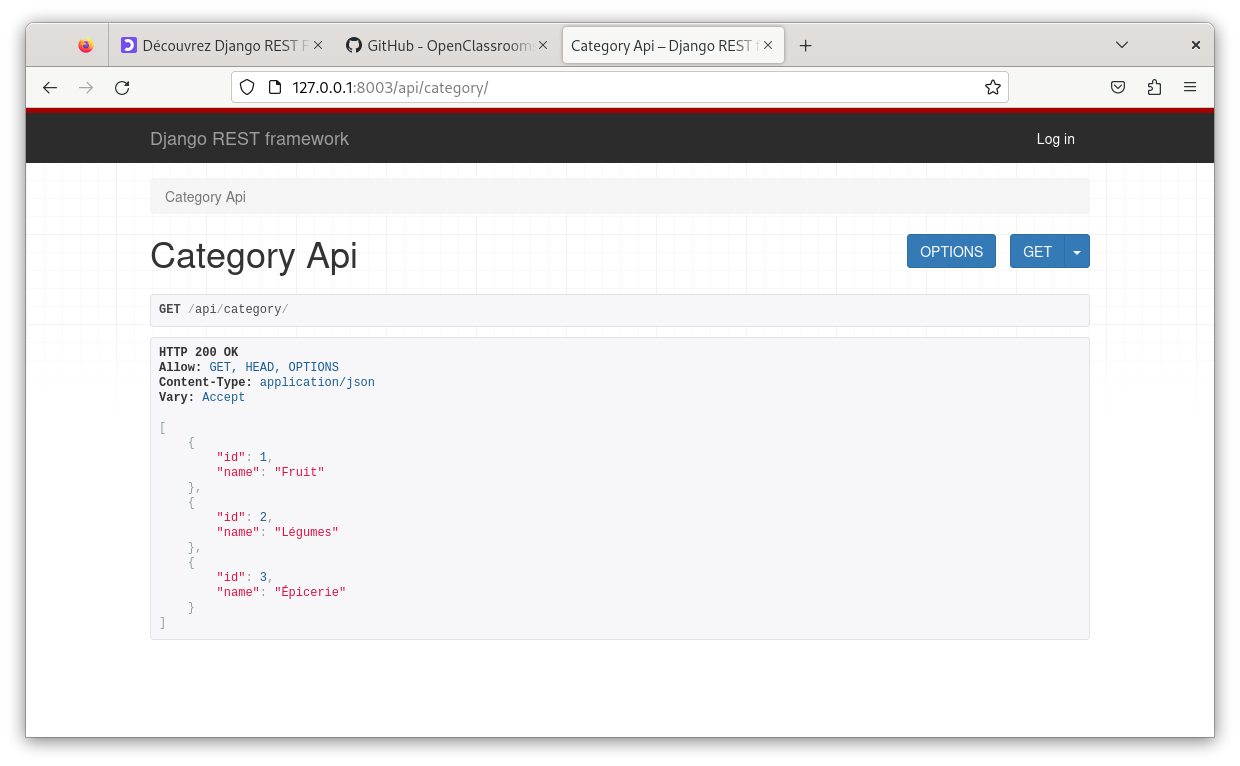
\includegraphics[width=15cm]{images/image05.png}
\end{center}

N’hésitez pas à jouer avec notre nouveau serializer, lui ajouter des champs, comme les dates de création et de modification. Tentez l’écriture pour les autres méthodes HTTP, l’expérimentation est un levier !

\subsection{Découvrez les méthodes d’un {\color{monOrange}endpoint}}
Seul {\color{monOrange}GET} est accessible sur notre endpoint, car nous n’avons redéfini que la méthode  {\color{monOrange}get}  dans la {\color{monOrange}View}. Ne pas réécrire de méthodes permet de ne pas les rendre accessibles. Nous pourrions réécrire également les méthodes  {\color{monOrange}post,  patch}  et  {\color{monOrange}delete}. 

\subsubsection{{\tt GET} et {\tt POST} servent avec Django à créer de nouvelles entités au travers de formulaires, mais {\tt PATCH} et {\tt DELETE} servent à quoi ?}
Reprenons-les une par une pour voir réellement à quoi servent ces méthodes HTTP dans le cadre d’une API, et les différences avec un site Internet classique :
\begin{itemize}
\item {\color{monOrange}GET} : Permet la lecture d'informations.
Un peu comme un site Internet classique, les appels en GET renvoient des données qui sont généralement du HTML qui est lu et rendu dans le navigateur. Dans le cas d’une API, il s’agit de JSON.
\item {\color{monOrange}POST} : Permet la création d’entités.
Alors que sur un site les appels en POST peuvent être utilisés pour modifier une entité, dans le cas d’une API, les POST permettent la création.
\item {\color{monOrange}PATCH} : Permet la modification d’une entité.
PATCH permet la modification de tout ou partie des valeurs des attributs d’une entité pour une API, alors que pour un site classique, nous utilisons un formulaire et un POST.
\item {\color{monOrange}DELETE} : Permet la suppression d’une entité.
DELETE permet la suppression d’une entité pour une API, alors que pour un site classique, nous utilisons un formulaire et généralement un POST.
\item {\color{monOrange}PUT} : Permet également la modification d’une entité.
Il est peu utilisé en dehors de l’interface de DRF, que nous verrons ensuite. Pour un site classique, l’action de modification entière d’une entité passe également par un POST au travers d’un formulaire.
\end{itemize}

Pas de panique, tout n’est pas à retenir tout de suite. Durant ce cours, nous allons aborder chacune de ces méthodes dans divers cas pratiques.

Ce qui est important à retenir est que chaque méthode correspond à une action du CRUD (Create, Read, Update, Delete), et c’est cela qui va nous permettre d’agir directement sur nos models.

\subsubsection*{Exercice}
Je vous propose de prendre la main et de mettre en place un nouvel endpoint qui va permettre de lister tous les produits de notre boutique en ligne. Utilisons l’URL suivante : \url{http://127.0.0.1:8000/api/product/}. Cet endpoint doit retourner les informations suivantes des produits :
\begin{itemize}
\item Son identifiant  {\tt id}.
\item Sa date de création  {\tt date\_created}.
\item Sa date de modification  {\tt date\_updated}.
\item Son nom  {\tt name}.
\item L’identifiant de la catégorie à laquelle il appartient  {\tt category}.
\end{itemize}
Pour réaliser cela, vous pouvez partir de la branche \href{https://github.com/OpenClassrooms-Student-Center/7192416\_APIs\_DRF/tree/P1C3\_exercice}{P1C3\_exercice}. Elle contient déjà ce que nous venons de faire ensemble. Une solution est proposée sur la branche \href{https://github.com/OpenClassrooms-Student-Center/7192416\_APIs\_DRF/tree/P1C3\_solution}{P1C3\_solution}.

\subsubsection*{En résumé}
\begin{enumerate}
\item Le fonctionnement des serializers proposé par DRF est similaire à celui des formulaires de Django.
\item Les serializers permettent de faire une représentation de nos models en JSON.
\item Les méthodes HTTP utilisables sont la représentation du CRUD (Create, Read, Update, Delete).
\item DRF nous propose une interface web qui permet de visualiser notre API.
\end{enumerate}
N’hésitez pas à modifier les données que retournent le serializer. Imaginez le but de l’endpoint que vous êtes en train de mettre en place pour déterminer quelles sont les données les plus pertinentes à retourner.
\section{Rendez les Views plus génériques avec un ModelViewset}
\section{Mettez en place un {\color{monOrange}router}}
Plutôt que de créer nos URL et de redéfinir nos méthodes une à une, DRF propose des classes héritables pour nos vues, qui sont les {\color{monOrange}ModelViewsets}. Elles permettent la mise en place rapide de toutes les actions du CRUD pour un model donné. Utiliser un ModelViewset nécessite d’utiliser une autre façon de définir nos URL. Cela se fait au travers d’un {\color{monOrange}router}.
\subsection*{Un router, c’est quoi ?}
Un router permet de définir automatiquement toutes les URL accessibles pour un endpoint donné. Il va à la fois permettre de définir :
\begin{itemize}
\item L’URL  {\tt /api/category/}, qui permet de réaliser des actions globales qui ne concernent pas directement une entité précise, comme la récupération de la liste des entités ou la création d’une nouvelle.
\item L’URL  {\tt /api/category/<pk>/}, qui en acceptant un paramètre correspondant à l’identifiant d’une entité, va permettre de réaliser des actions sur celle-ci, comme obtenir des informations, la modifier ou la supprimer.
\end{itemize}
{\em Mettons en place notre {\color{monOrange}router}} dans notre fichier {\tt urls.py}  et supprimons notre ancien {\color{monOrange}endpoint}: 
\begin{minted}[
mathescape,
framesep=2mm,
baselinestretch=1.2,
%fontsize=\footnotesize,
bgcolor=LightGray,
%linenos
]{python}
from django.contrib import admin
from django.urls import path, include
from rest_framework import routers
from shop.views import CategoryViewset
 
# Ici nous créons notre routeur
router = routers.SimpleRouter()
# Puis lui déclarons une url basée sur le mot clé ‘category’ et notre view
# afin que l’url générée soit celle que nous souhaitons ‘/api/category/’
router.register('category', CategoryViewset, basename='category')
 
urlpatterns = [
    path('admin/', admin.site.urls),
    path('api-auth/', include('rest_framework.urls')),
    path('api/', include(router.urls))  # Il faut bien penser à ajouter les 
    # urls du router dans la liste des urls disponibles.
]
\end{minted}
Le router se définit en amont de la définition de  {\tt urlpatterns}. Les URL sont incluses avec un  {\tt include}  au travers de la propriété  {\tt router.urls}. Notons également qu’il n’est plus nécessaire d'appeler  {\tt .as\_view()}, le router le fait pour nous lorsqu’il génère les URL.

\begin{theorem}
Le paramètre {\tt basename}  permet de retrouver l’URL complète avec la fonction {\tt redirect}, comme le propose Django. Cela sera utile lors de l’écriture des tests que nous aborderons ensuite.
\end{theorem}

\subsection{Transformez une ApiView en ModelViewset}
À présent, nous devons transformer notre  {\color{monOrange}ApiView}  en un  {\color{monOrange}ModelViewset} pour que notre vue puisse être connectée à notre routeur. Un {\color{monOrange}ModelViewset}  est comparable à une super vue Django qui regroupe à la fois {\color{monOrange}CreateView, UpdateView, DeleteView, ListView}  et {\color{monOrange}DetailView}. Il faut impérativement lui {\em définir deux attributs de classe }:
\begin{enumerate}
\item {\tt serializer\_class}  qui va déterminer le {\tt serializer} à utiliser ;
\item {\tt queryset}, ou réécrire la méthode {\tt get\_queryset}  qui doit retourner un {\color{monOrange}Queryset} des éléments à retourner.
\end{enumerate}
\begin{theorem}
Redéfinir seulement l’attribut de classe {\tt queryset}  permet principalement de faire des tests rapides. À l’usage, redéfinir {\tt get\_queryset}  est souvent la solution à adopter car elle permet d’être plus fin sur les éléments à retourner.
\end{theorem}
\begin{minted}[
mathescape,
framesep=2mm,
baselinestretch=1.2,
%fontsize=\footnotesize,
bgcolor=LightGray,
%linenos
]{python}
from rest_framework.viewsets import ModelViewSet
from shop.models import Category
from shop.serializers import CategorySerializer
 
class CategoryViewset(ModelViewSet):
 
    serializer_class = CategorySerializer
 
    def get_queryset(self):
        return Category.objects.all()
\end{minted}
Nous pouvons dès à présent retester notre API à l’adresse \url{http://127.0.0.1:8000/api/category/}.
Le résultat est identique à ce que nous avions précédemment. La différence étant qu’il nous est maintenant possible de réaliser directement les autres opérations du {\color{monOrange}CRUD}. Le formulaire en bas de page vous invite directement à réaliser un {\color{monOrange}POST} pour créer une nouvelle catégorie.
\begin{center}
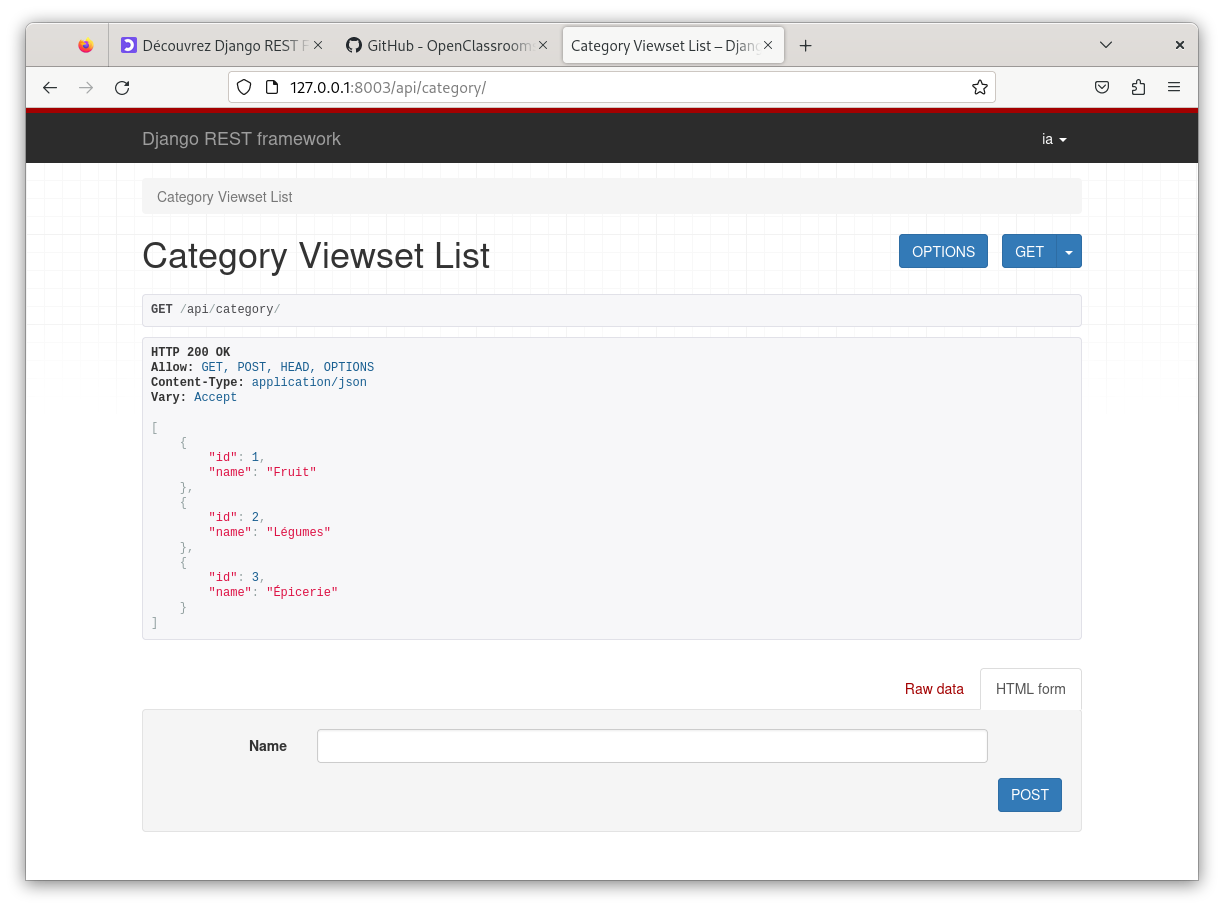
\includegraphics[width=10cm]{images/image06.png}
\end{center}
Le détail d’une catégorie est également visible en ajoutant son identifiant dans l’URL, par exemple \url{http://127.0.0.1:8000/api/category/1/}. La page vous propose alors de réaliser les actions {\color{monOrange}PUT, PATCH} (dans l’onglet « Raw data ») et {\color{monOrange}DELETE} sur l’entité consultée.
\begin{center}
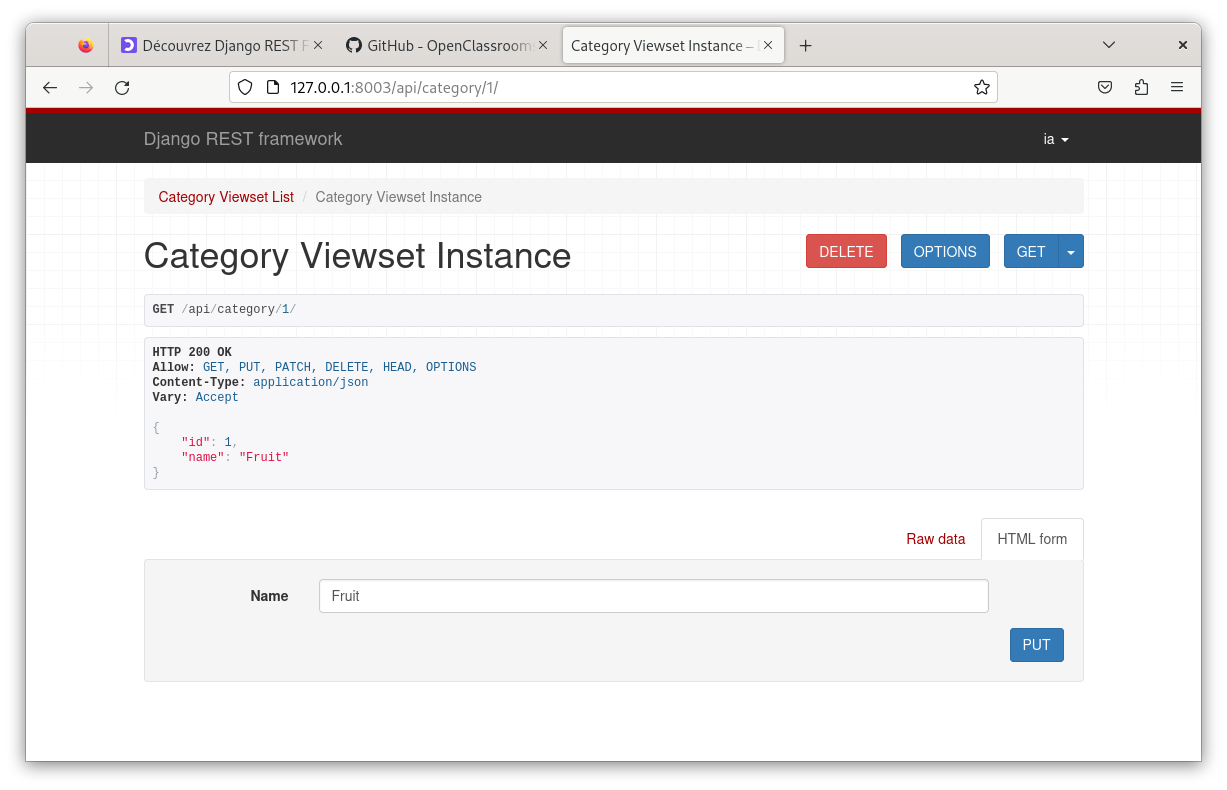
\includegraphics[width=10cm]{images/image07.png}
\end{center}
\subsection{Ne permettez que la lecture}
Vous l’aurez sûrement remarqué, nous pouvons créer de nouvelles catégories ; dans la pratique, permettre la création, la modification et la suppression sur un endpoint public comme le nôtre n’est pas conseillé. Nous allons donc faire en sorte que notre endpoint {\em ne permette que la lecture}, car son but est d’afficher à nos utilisateurs la liste des catégories disponibles sur la boutique. Pour cela, DRF nous propose un autre type de {\color{monOrange}ModelViewset}. Il s’agit du {\color{monOrange}ReadOnlyModelViewset}  qui, comme son nom l’indique, ne permet que la lecture.

Modifions notre vue pour limiter les opérations disponibles. Nous allons faire étendre la vue CategoryViewset  avec le {\tt viewset} {\color{monOrange}ReadOnlyModelViewset}   au lieu du {\color{monOrange}ModelViewset}  actuel.
\begin{minted}[
mathescape,
framesep=2mm,
baselinestretch=1.2,
%fontsize=\footnotesize,
bgcolor=LightGray,
%linenos
]{python}
from rest_framework.viewsets import ReadOnlyModelViewSet
from shop.models import Category
from shop.serializers import CategorySerializer
 
class CategoryViewset(ReadOnlyModelViewSet):
    serializer_class = CategorySerializer
    def get_queryset(self):
        return Category.objects.all()
\end{minted}
Si nous consultons à présent notre API, nous pouvons constater que toutes les options autres que la lecture ne sont plus permises.
\begin{center}
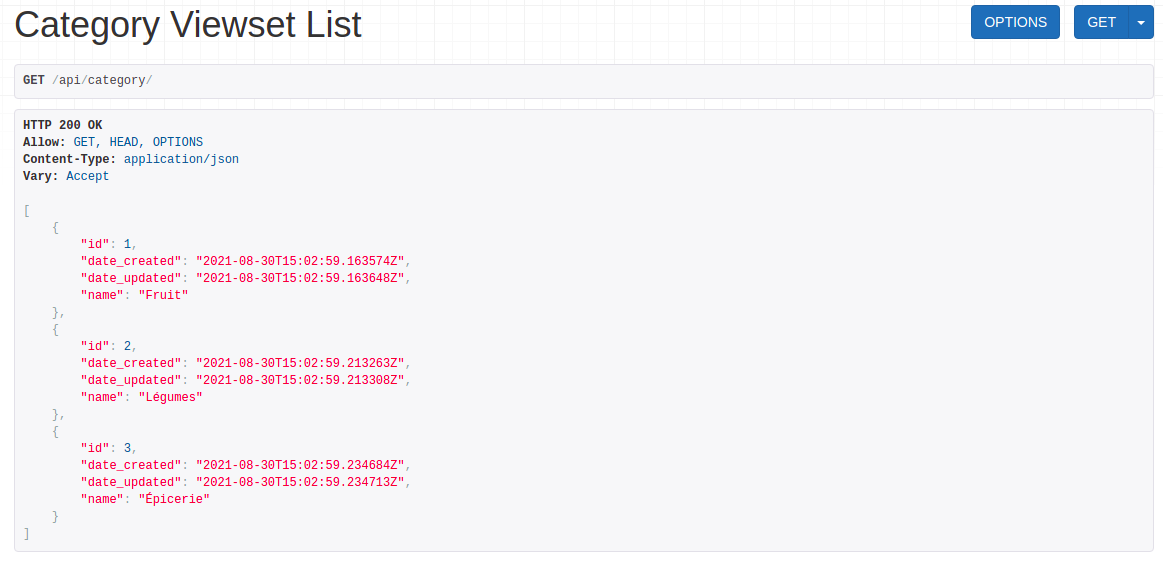
\includegraphics[width=10cm]{images/image08.png}
\end{center}
\begin{theorem}
Il est également possible d’utiliser l’attribut   {\tt read\_only\_fields}  sur le serializer pour préciser les champs en lecture seule. Mais cela n'empêchera pas les actions de création, modification et suppression.
\end{theorem}
\subsubsection*{Exercice}
Notre endpoint de consultation de produits ne doit également permettre que la lecture. Entraînez-vous dans l’utilisation des Viewsets  pour passer cet endpoint en « lecture seule ».
\begin{itemize}
\item Pour réaliser cela, vous pouvez partir de la branche \href{https://github.com/OpenClassrooms-Student-Center/7192416\_APIs\_DRF/tree/P1C4\_exercice}{P1C4\_exercice}. Elle contient déjà ce que nous venons de faire ensemble.
\item Une solution est proposée sur la branche \href{https://github.com/OpenClassrooms-Student-Center/7192416\_APIs\_DRF/tree/P1C4_solution}{P1C4\_solution}.
\end{itemize}
\subsubsection*{En résumé}
\begin{enumerate}
\item Un router permet de définir en une seule fois toutes les opérations du CRUD sur un endpoint.
\item Utiliser un  {\tt ModelViewset}  impose d’utiliser un router pour définir ses URL.
\item Lors de l’utilisation d’un {\tt ModelViewset}, il faut définir :
\begin{enumerate}
\item le serializer à utiliser avec l’attribut de classe {\tt serializer\_class}  ;
\item le jeu de données qui sera retourné en réécrivant la méthode {\tt get\_queryset}.
\end{enumerate}
\item {\tt ReadOnlyModelViewset}  permet de limiter les accès à la lecture seule.
\end{enumerate}
{\em Les Viewsets sont très souvent les vues à privilégier, nous allons dès maintenant voir comment les personnaliser et les adapter avec plus de précision à nos besoins. Suivez-moi au prochain chapitre !}

\section{Filtrez les résultats d’un endpoint}
\subsection{Appliquez un filtre sur les données retournées}
Lorsque nos utilisateurs naviguent sur notre boutique, il se peut qu’ils souhaitent récupérer les produits d’une catégorie grâce à un appel fait à notre API. Sauf que pour le moment, notre endpoint de produits ne permet pas de {\em filtrer par catégorie}. Pour réaliser cela, nous allons accepter un paramètre dans l’URL qui sera l’identifiant de la catégorie, pour ne renvoyer que les produits correspondants. Le paramètre sera nommé {\tt category\_id}, ce qui donnera une URL sous le format
\begin{center}
\url{http://127.0.0.1:8000/api/product/?category_id=1}.
\end{center}
Éditons notre classe {\tt ProductViewset}  pour qu’elle applique un nouveau filtre si le paramètre est présent. Profitons-en pour également appliquer le filtre sur les produits actifs :
\begin{minted}[
mathescape,
framesep=2mm,
baselinestretch=1.2,
%fontsize=\footnotesize,
bgcolor=LightGray,
%linenos
]{python}
class ProductViewset(ReadOnlyModelViewSet):
    serializer_class = ProductSerializer
    def get_queryset(self):
    # Nous récupérons tous les produits dans une variable nommée queryset
        queryset = Product.objects.filter(active=True)
        # Vérifions la présence du paramètre ‘category_id’ dans l’url et si oui alors appliquons notre filtre
        category_id = self.request.GET.get('category_id')
        if category_id is not None:
            queryset = queryset.filter(category_id=category_id)
        return queryset
\end{minted}

À présent, nous pouvons constater que le filtre est bien appliqué si nous consultons la liste des produits de la catégorie 1 avec l’URL 

\begin{center}
\url{http://127.0.0.1:8000/api/product/?category_id=1}.
\end{center}
\begin{center}
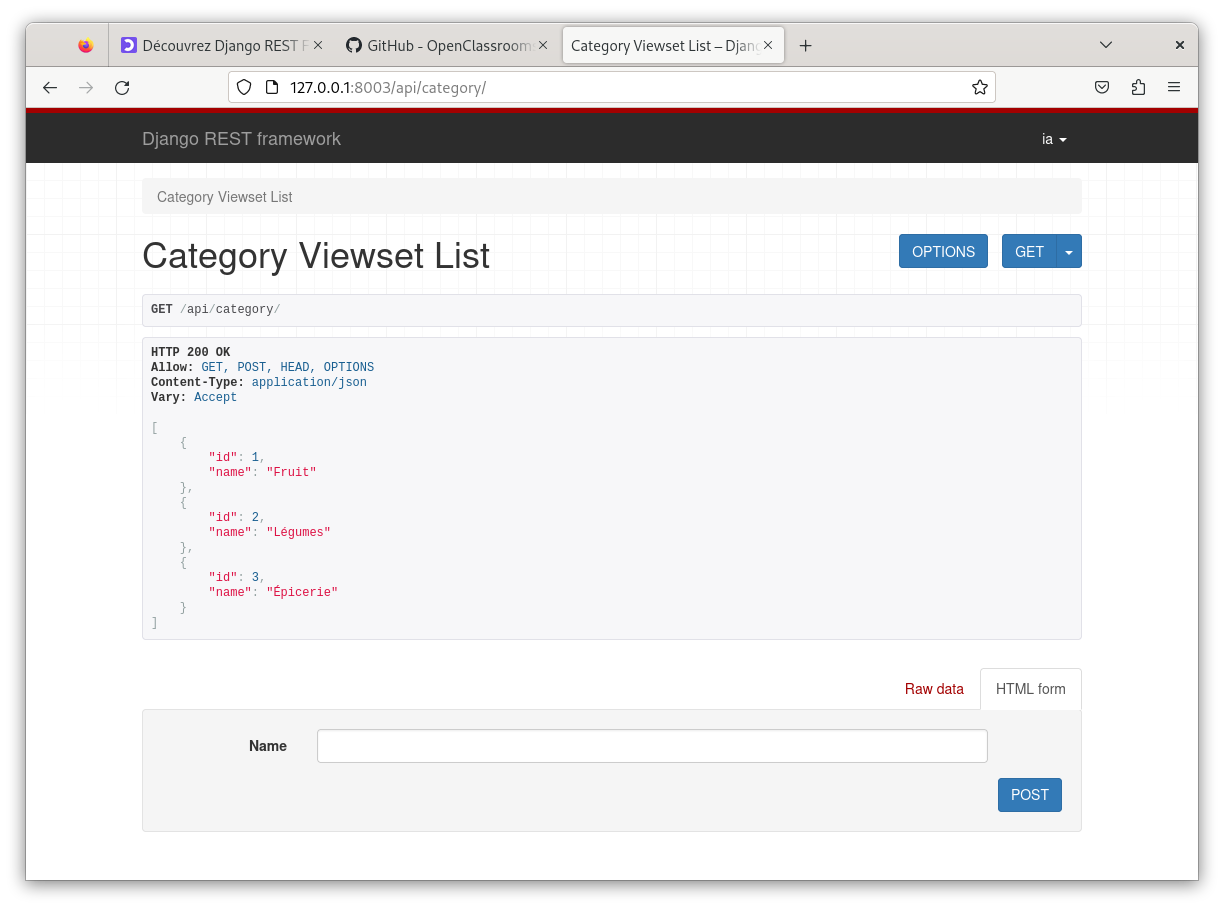
\includegraphics[width=10cm]{images/image09.png}
\end{center}
Et si nous demandons une catégorie qui n'existe pas, alors une liste de produits vide est retournée sans faire planter notre application :
\begin{center}
\url{http://127.0.0.1:8000/api/product/?category_id=7777777}.
\end{center}
\begin{center}
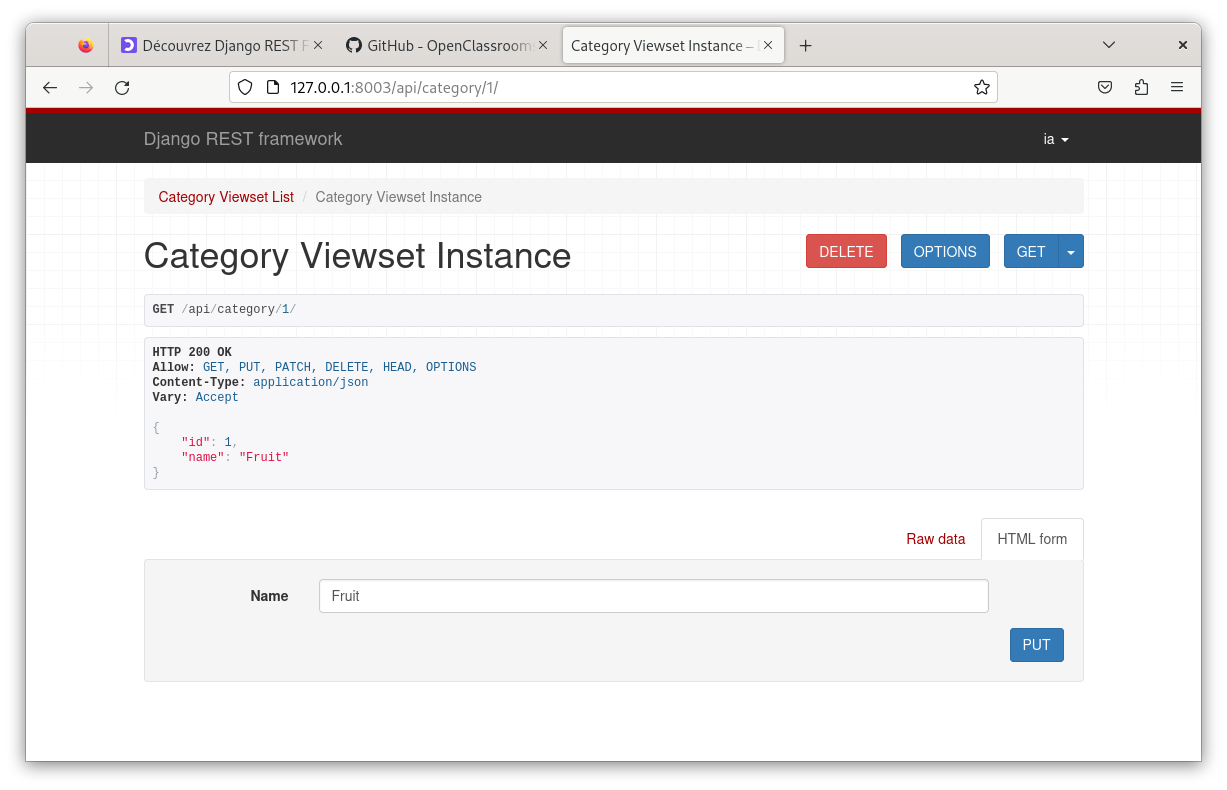
\includegraphics[width=10cm]{images/image10.png}
\end{center}

Ainsi, les paramètres d’URL peuvent servir à appliquer {\em toutes sortes de filtres sur les données retournées}. N’hésitez pas à jouer avec, en permettant par exemple de forcer l’affichage des produits inactifs.
\begin{theorem}
Nous aurions pu améliorer encore notre endpoint, en lui ajoutant un paramètre permettant d’inclure les catégories non disponibles, par exemple. N’hésitez pas à les utiliser, ils sont souvent une solution qui évite la création d’un nouvel endpoint.
\end{theorem}

\subsubsection*{Exercice}
À votre tour ! Pour parfaire notre boutique, nous souhaitons mettre en place un endpoint de récupération des articles sur l’URL http://127.0.0.1:8000/api/article/. Il ne doit retourner que les articles actifs, et permettre de filtrer les articles retournés sur une catégorie avec un paramètre {\tt product\_id}.
Cet endpoint doit retourner les informations suivantes :
\begin{itemize}
\item L’identifiant de l’article ;
\item La date de création et de modification de l’article ;
\item Le nom de l’article ;
\item Le prix de l’article ;
\item L’identifiant du produit auquel appartient l’article.
\end{itemize}
Pour réaliser cela, vous pouvez partir de la branche \href{https://github.com/OpenClassrooms-Student-Center/7192416\_APIs\_DRF/tree/P1C5\_exercice}{P1C5\_exercice}. Elle contient déjà ce que nous venons de faire ensemble. Une solution est proposée sur la branche \href{https://github.com/OpenClassrooms-Student-Center/7192416\_APIs\_DRF/tree/P1C5\_solution}{P1C5\_solution}.

\subsubsection*{En résumé}
\begin{enumerate}
\item Redéfinir la méthode {\tt get\_queryset}  permet de définir les entités à prendre en compte dans l'endpoint.
\item Il est possible d’utiliser des paramètres d’URL pour apporter des précisions sur l’action à réaliser (comme filtrer sur un critère particulier).
\end{enumerate}

{\em C’est maintenant l’heure d’écrire les premiers tests pour notre API ! Rendez-vous au prochain chapitre.}

\section{Écrivez des tests pour votre API}
\subsection{Découvrez le TestCase de DRF}
Les tests sont un élément important de tout projet de développement. Ils permettent de garantir la pérennité du projet, sa maintenance, et surtout de déployer la conscience plus tranquille.

Une nouvelle classe de test {\color{monOrange}APITestCase}  est fournie par DRF. Elle est faite pour fonctionner de la même façon que la classe {\color{monOrange}TestCase}. Sa principale différence étant d’utiliser un client qui permet une utilisation plus simple des appels. Il est donc recommandé de l’utiliser pour ne pas avoir à définir plusieurs paramètres pour réaliser nos appels lors des tests.

\subsection{Écrivez des tests avec APITestCase}
Créons notre fichier de test dans l’application {\tt shop}  et mettons en place un test qui {\em vérifie l’endpoint de récupération des catégories actives}. Nous allons pour cela :
\begin{itemize}
\item Créer deux catégories dont une inactive ;
\item Réaliser notre appel ;
\item Vérifier que le status code de la réponse est bien un succès : 200 ; 
\item Nous assurer que le contenu de la réponse est bien celui attendu, et qu'il ne comprend pas la catégorie désactivée.
\end{itemize}
Nous écrirons aussi un test qui s’assurera que la création d’une catégorie n’est pas possible, et tombe bien en erreur.
\begin{theorem}
Il est très facile d’oublier d’écrire des tests pour les cas positifs en erreur. Notre API étant pour le moment publique, il est important de tester qu’un utilisateur ne puisse pas créer de nouvelles catégories.
\end{theorem}
Créons d'abord un fichier  {\tt tests.py}  pour nos tests. Puis, c’est parti pour nos deux tests :
\begin{minted}[
mathescape,
framesep=2mm,
baselinestretch=1.2,
fontsize=\footnotesize,
bgcolor=LightGray,
%linenos
]{python}
from django.urls import reverse_lazy
from rest_framework.test import APITestCase

from shop.models import Category

class TestCategory(APITestCase):
    # Nous stockons l’url de l'endpoint dans un attribut de classe pour pouvoir
    # l’utiliser plus facilement dans chacun de nos tests
    url = reverse_lazy('category-list')

    def format_datetime(self, value):
        # Cette méthode est un helper permettant de formater une date en chaine de caractères 
        # sous le même format que celui de l’api
        return value.strftime("%Y-%m-%dT%H:%M:%S.%fZ")

    def test_list(self):
        # Créons deux catégories dont une seule est active
        category = Category.objects.create(name='Fruits', active=True)
        Category.objects.create(name='Légumes', active=False)

        # On réalise l’appel en GET en utilisant le client de la classe de test
        response = self.client.get(self.url)
        # Nous vérifions que le status code est bien 200
        # et que les valeurs retournées sont bien celles attendues
        self.assertEqual(response.status_code, 200)
        excepted = [
            {
                'id': category.pk,
                'name': category.name,
                'date_created': self.format_datetime(category.date_created),
                'date_updated': self.format_datetime(category.date_updated),
            }
        ]
        self.assertEqual(excepted, response.json())

    def test_create(self):
        # Nous vérifions qu’aucune catégorie n'existe avant de tenter d’en créer une
        self.assertFalse(Category.objects.exists())
        response = self.client.post(self.url, data={'name': 'Nouvelle catégorie'})
        # Vérifions que le status code est bien en erreur et nous empêche de créer une catégorie
        self.assertEqual(response.status_code, 405)
        # Enfin, vérifions qu'aucune nouvelle catégorie n’a été créée malgré le status code 405
        self.assertFalse(Category.objects.exists())
\end{minted}

\begin{theorem}
Lors d’un développement, il vaut mieux prendre le temps d’écrire les tests au fil de l’eau, ce qui est moins décourageant que de les écrire tous à la fin. Parfois il peut aussi être intéressant de commencer par écrire le test avant de développer la fonctionnalité.
\end{theorem}
\subsubsection*{Exercice}
Écrivez vous aussi des tests pour l’endpoint de produits. Il peut également être intéressant de créer une classe de test pour notre projet, contenant notre méthode d’aide au formatage de date, qui sera étendu par nos classes de tests.
\begin{itemize}
\item Mettez en place une classe {\tt ShopAPITestCase}.
\item Refactorisez  {\tt TestCategory}  pour qu’elle étende notre nouvelle classe  {\tt ShopAPITestCase}.
\item Écrivez la classe de test  {\tt TestProduct}  qui va tester :
\begin{itemize}
\item l’endpoint de liste et de détail d’un produit ;
\item que le filtre sur la liste fonctionne correctement ;
\item qu’il n’est pas possible de créer, modifier et supprimer un produit.
\end{itemize}
\end{itemize}
Pour réaliser cela, vous pouvez partir de la branche \href{https://github.com/OpenClassrooms-Student-Center/7192416\_APIs\_DRF/tree/P1C6\_exercice}{P1C6\_exercice}. Elle contient déjà ce que nous venons de faire ensemble. Une solution est proposée sur la branche \href{https://github.com/OpenClassrooms-Student-Center/7192416\_APIs\_DRF/tree/P1C6\_solution}{P1C6\_solution}.

\subsubsection*{En résumé}
\begin{enumerate}
\item DRF met à disposition une classe de tests qu’il faut utiliser pour tester une API.
\item Il est important de tester le status code de retour ainsi que le contenu de la réponse.
\item Ne pas oublier de tester les cas d’erreur.
\item Les tests ne sont pas la partie la plus intéressante à écrire, mais ils garantissent la stabilité d’un projet dans le temps.
\end{enumerate}
{\em Nous voilà avec une API DRF simple et validée par nos premiers tests ! Avant de passer à l’étape suivante, validez vos acquis dans le quiz de la partie 1 – je vous attends dans la partie 2 !}




\end{document}










